\providecommand{\isolatedBuild}[1]{#1}% fallback definition lets this file build normally
\isolatedBuild
{
\documentclass[11pt,letterpaper]{book}
\usepackage{import}

% This file must be found via the TEXINPUTS environment variable.
%\documentclass[11pt,letterpaper]{book}

% aleeper: I think these are needed for Paul's macros?
\usepackage{epsfig}
\usepackage{epstopdf}

%\makeatletter
%\typeout{The import path is \import@path}
%\makeatother

\usepackage{import}

\subimport{./}{packagesMitiguy.sty}
\subimport{./}{macrosMitiguy.tex}
\subimport{./}{PageStylesMitiguy.tex}
\subimport{./}{macrosLeeper.tex}


\pagestyle{empty}
\pagenumbering{arabic}

\begin{document}
\HandoutHeader{Vector Equations and Geometry}
\normalsize
\vspace{-1.5pc}
\\[0.0pc]
%
%\begin{enumerate}
%\item
\textbf{\ \ }\textColorBold{darkerBlue}{Distance between point and plane}
\\[0.5pc]
%\graphicspath{{../problems/VectorGeometry/}}
%\input ../problems/VectorGeometry/first_and_ten.tex
}
%%%%%%%%%%%%%%%%%%%%%%%%%%%%%%%%%%%%%%%%%%%%%%%%%%%%%%%%%%%
%
\begin{minipage}[t]{\columnwidth}
%
\begin{minipage}[t]{0.6\columnwidth}
A common problem in many fields is to determine what side of an oriented plane a point lies on.
%
As an example from structural design, consider the triangular skylight window shown. Point $P$ is at one corner of the window, with $\posvec{A_o}{P} =  4~\uvecx{a}$. A (non-unit) vector perpendicular to the window, pointing ``outward,'' is
$\bvec{n} =  1~\uvecx{a} + 1~\uvecy{a} + 1~\uvecz{a}$.
%\\[0.0pc]$\posvec{A_o}{P} =  1~\uvecx{a}$
%\\[0.0pc]$\arrowVector{n} =  1~\uvecx{a} + 1~\uvecy{a} + 1~\uvecz{a}$
\\[0.5pc]
An exterior rigid structure (not shown) is planned to be positioned near the window.
It has been determined that the point of the structure nearest the window,
which we will call point $Q$,
will be at $\posvec{A_o}{Q} =  2~\uvecx{a} + 2~\uvecy{a} + 1~\uvecz{a}$.
\end{minipage}
%
\hfill
%
\begin{minipage}[t]{0.3\columnwidth}
\vspace*{0.1cm}
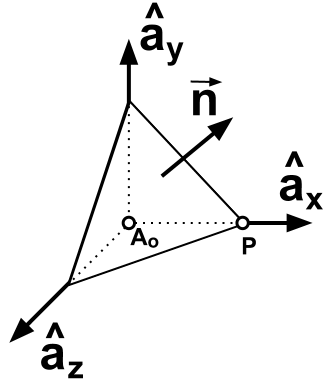
\includegraphics[width=\columnwidth]{point_plane.png}
\end{minipage}
%
\end{minipage}
\\[0.5pc]
%
Determine if point $Q$ (and hence, the whole structure) will remain clear of the window.
That is, does $Q$ lie ``outside/above'' the window (in the direction of \bvec{n})?
You must clearly explain how any numerical result you get implies one answer or the other.
\\[0.25pc]\textbf{Hint:} Write down \posvec{P}{Q}.
\\[1.0pc]
\isolatedBuild {
%\end{enumerate}
\vfill \end{document} }
